\subsubsection{File Splitting Analysis}
The purpose of this section is to run some analysis on the performance benefits of splitting up sound files into smaller portions. As mentioned above, sixty minute, 1.29GB sound files are too large to compute even on high end systems. Thus, some research must be done to find the most efficient format for processing. The following results are all ACI index run using System 1, and on the same sound file from the Benchmarking section above. Keep in mind that the ACI index could not be processed on System 1 using the sixty minute file due to memory constraints.\\

\noindent\textbf{One Minute Splits}\\
The analysis took 2.45 seconds to process a the first minutes of the wav sound file. The analysis took 2.48 seconds to process the next minute of the wav sound file. Thus, it is assumed that these splits all come out to around two and a half seconds of processing time per minute. To do the whole sixty minutes, it would take about two minutes and thirty seconds using one minute splits.\\

\noindent\textbf{Five Minute Splits}\\
The analysis took 14.15 seconds to process a the first five minutes of the wav sound file. The analysis took 14.06 seconds to process the next five minutes of the wav sound file. Thus, it is assumed that these splits all come out to around fourteen seconds of processing time per five minutes. To do the whole sixty minutes, it would take about two minutes and fourty eight seconds using five minute splits.\\

\noindent\textbf{Ten Minute Splits}\\
The analysis took 30.09 seconds to process a the first ten minutes of the wav sound file. The analysis took 29.00 seconds to process the next ten minutes of the wav sound file. Thus, again it can be assumed that these splits all come out to around thirty seconds of processing time per ten minutes. To do the whole sixty minutes, it would take about three minutes using ten minute splits.\\

\noindent\textbf{Fifteen Minute Splits}\\
The analysis took 44.20 seconds to process a the first fifteen minutes of the wav sound file. The analysis took 43.51 seconds to process the next fifteen minutes of the wav sound file. Thus, it can be assumed that these splits all come out to around forty four seconds of processing time per fifteen minutes. To do the whole sixty minutes, it would take about two minutes and fifty four seconds using fifteen minute splits.\\

\noindent\textbf{Twenty Minute Splits}\\
The analysis took 59.46 seconds to process a the first twenty minutes of the wav sound file. The analysis took 58.54 seconds to process the next twenty minutes of the wav sound file. Thus, it can be assumed that these splits all come out to around fifty nine seconds of processing time per twenty minutes. To do the whole sixty minutes, it would take about two minutes and fifty seven seconds using twenty minute splits.\\

\noindent\textbf{Thirty Minute Splits}\\
The analysis took 134.63 seconds to process a the first thirty minutes of the wav sound file. The analysis took 117.55 seconds to process the last thirty minutes of the wav sound file. This is a range of about seventeen seconds, so best case scenario we are looking at just under two minutes for thirty seconds. To do the whole sixty minutes, it would take about three minutes and fifty five seconds using thirty minute splits. This is much higher than all the other splits, which comes as a surprise.\\

\noindent\textbf{Conclusions}\\
\begin{center}
	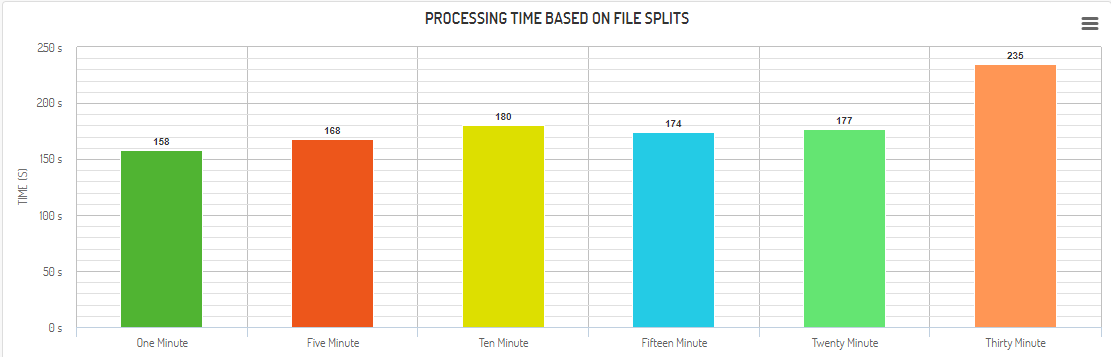
\includegraphics[width=\textwidth]{fileSplits}
\end{center}
Interestingly, all the different splits performed mostly the same \textit{except} for the thirty minute splits. Further, the ten minute splits ended up a tad bit higher than even the fifteen and twenty minute splits. The lowest recorded time was the one minute splits, and the highest being the thirty minute splits. Going forward, this research helps us make the decision on how to split the files up to maximize performance, especially on lower end systems. It seems that one to five minute splits will be the best choice.
